\chapter{System Analysis and Feasibility}

The goal of the project is to develop a model for cloud detection based on U-Net architecture which uses Convolutional Neural Network. In this regard, feasibility studies were conducted.
\section{Feasibility}
\subsection{Time Feasibility}

A three-month period was determined to be proper for project completion. The Waterfall approach was used to create the time feasibility aspect.

Gannt Schema for the project is given below at Figure \ref{gannt}.
\begin{figure}[htp]
    \centering
    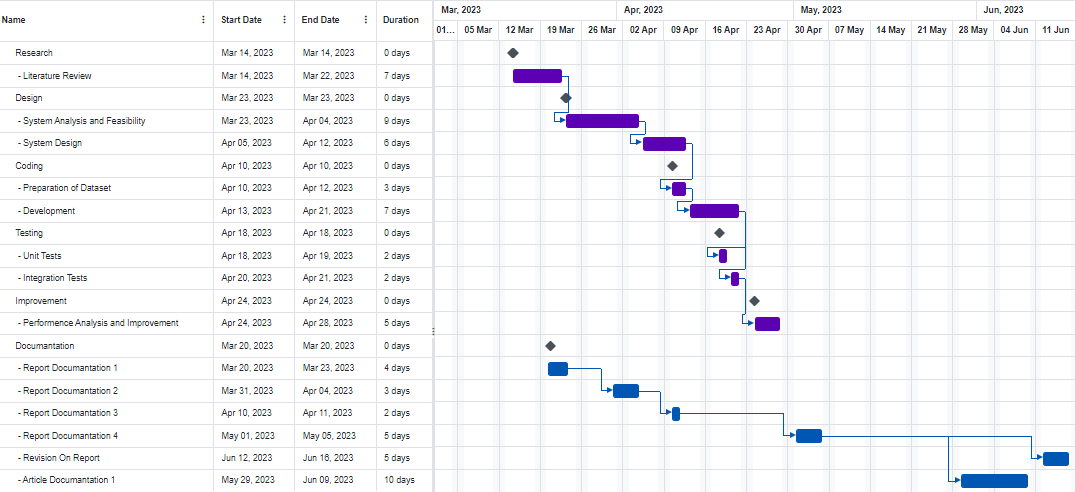
\includegraphics[width=15cm]{projectChapters/images/gannt.png}
    \caption{Gantt Schema for Project}
    \label{gannt}
\end{figure}

\subsection{Technical Feasibility}

\subsubsection{Hardware Feasibility}

The initial work on training the model was done on Google Colab and a draft was
created. However, due to GPU and time limitations in the free trial of Colab, the
training of the entire dataset was done on our local machine. The dataset contains a
total of 16GB of data and the specifications of the computer needs to create the model
are as follows:

\begin{itemize}
    \item  Hard Drive: ADATA SX8100NP M2 SSD
    \item  Processor: AMD Ryzen 5600X 6-Core
    \item  Graphics: NVIDIA GeForce RTX 3060 Ti
    \item  RAM: 32GB
\end{itemize}

The least specifications above are sufficient for training and usage. Two computer which has the specifitacations were needed for the project.

\subsubsection{Software Feasibility}

Python language was preferred for model training. The use of libraries such as TensorFlow, Matplotlib, scikit-image, NumPy, and Hub, as well as their user-friendly interfaces, validates their inclusion in the project. Tensorflow library was used for the design of the model. Python version 3.9.16 and compatible library versions were selected.

\subsection{Legal Feasibility}

The project's goal is to offer an approach for detecting clouds in satellite images. There is no need for an ethics committee's approval because the initiative does not include any possible damage or ethical issues. The dataset used is made up of Landsat 8 satellite images, which are freely available for public use and do not require any rights purchases. In terms of software licensing, open-source resources were used, and because the software was developed internally, no license rights were violated.
\hfill \break
\hfill \break
\subsection{Economic Feasibility}

The cost of the hardware used is 50.000 TL, since there are two computers with each one costing 25000. An employee works for 40.000 TL monthly. Two employees who work quarter-time for 4 days a week, paid 2 * 40.000 * 0.8 * 0.25 = 16.000. The payment for two individuals for 3 months is 16.000 * 3 = 48.000. So for this project total salary is calculated as 48,000 TL. The total budget is 50.000 + 48.000 = 98.000 TL

Costs of each components in a computer are given below at Table \ref{ch}.

\begin{table}[htp]
    \centering

    \begin{tabular}{ |p{6cm}||p{2cm}|}
     \hline
     \multicolumn{2}{|c|}{Hardware - Cost Table} \\
     \hline
     Component & Cost\\
     \hline
     \hline
     ADATA SX8100NP M2 SSD     &   1.500 TL\\
     \hline
     AMD Ryzen 5600X 6-Core   &     5.000 TL\\
     \hline
     NVIDIA GeForce RTX 3060 Ti  &  11.000 TL\\
     \hline
     32 GB RAM       &     2.500 TL\\
     \hline
     Other components for computer &   5.000 TL\\
     \hline
     \hline
     Total       &         25.000 TL\\
     \hline
    \end{tabular}

    \caption{Hardware - Cost Table for One Computer}
    \label{ch}
\end{table}


\section{Elements of the System}
The goal of this project is to create and implement an efficient cloud detection algorithm that simplifies the use of human, software, hardware, and data resources from satellite images.

The Table \ref{element} below provides an overview of the project's various resources, including hardware, software, human, and data resources.
\hfill \break
\begin{table}[htp]
    \centering

    \begin{tabular}{ |p{6cm}||p{6cm}|}
     \hline
     \multicolumn{2}{|c|}{Reasources} \\
     \hline
      Resource & Element\\
     \hline
     \hline
     Hardware Resources  & 2 Computer\\
     \hline
    Software Resources   &    Python - Jupyter Notebook\\
     \hline
     Human Resources  &  Şevval Bulburu
                         Mehmet Alperen Ölçer \\
     \hline
     Data Resources       &    Landsat 8 Satellite Images\\
     \hline
    \end{tabular}
    \caption{Resources which used for the project}
    \label{element}
\end{table}